\section{Implement Gradient Descent}
\subsection{Implementation the gradient Descent}
We implemented a function {\tt gradientDescent}  that takes the parameters:
\begin{enumerate}[-]
\item A scalar function $f: \mathbb{R}^n \mapsto \mathbb{R}$.
\item The gradient of $f$ $\nabla f: \mathbb{R}^n \mapsto \mathbb{R}^n$.
\item An initial guess $x_0 \in \mathbb{R}^n$.
\item A step size $s > 0$.
\item A convergence threshold $\epsilon > 0$.
\end{enumerate}
 {\tt gradientDescent} returns an array of $n+1$ numbers, corresponding to the $n$ coordinates of the current $x_t$, and the value of $f(x_t)$, for each of the steps $t$ before convergence of the algorithm.
 
 This choice of output lets us monitor the rate of convergence of the algorithm (which zones lead to slower or faster convergence), which will be useful when we compare different methods (see section \ref{comparison}). It also allows us to plot the path followed by the algorithm (see figures \ref{bowl} to \ref{bowls}). In all the figures that follow, we plot an initial guess (red dot) and a final result after gradient descent (blue dot). The blue line corresponds to the path followed by the gradient descent algorithm.

\subsection{Results and Impact of the choice of parameters}

We chose to benchmark our gradient descent on a variety of functions, designed to test all the potential cases that we might encounter. Because of plotting constraints, we focus the figures to function of two parameters:  $f: \mathbb{R}^2 \mapsto \mathbb{R}$.

\begin{figure}[h]
  \centering
 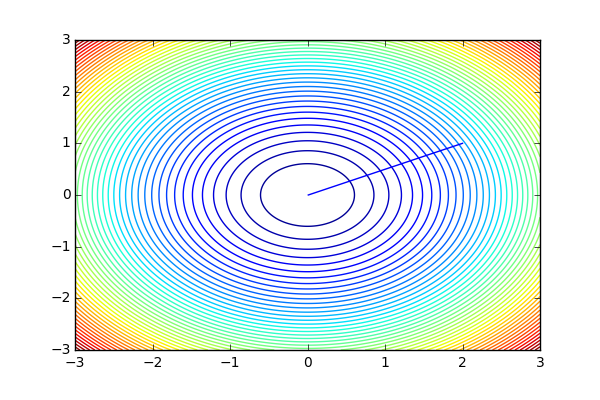
\includegraphics[width=4cm, height= 4cm]{../Figures/Q1/bowl.png}
\caption{$f : (x,y) \to 10x^2 + 10y^2$, $x_0 = (4,4)$, $s = 0.1$ and $\epsilon = 0.01$}
\label{bowl}
\end{figure}

In simple cases such as a quadratic bowl (figure \ref{bowl}), the convergence does not strongly depend on the choice of the parameters, and converges quite fast (here in 11 steps). Furthermore, there is no need to specify very small $s$ and $\epsilon$ to ensure convergence to the global maximum.

\subsubsection{Impact of the initial guess}

In the case of a very non convex function such as in figure \ref{normals} however, the choice of $x_0$ becomes important, and we see that even a slight perturbation in the original guess can lead to a totaly different result.
Another issue with highly non-convex functions is that the gradient descent may not even converge to a local minimum. For instance in figure \ref{normals}, for $x_0 = (1.5,1.5)$, the gradient at $x_0$ is $0$, therefore the algorithm is stuck at $x_0$.


In some cases (See figure \ref{nonconv}), the function does not have a minimum. This leads to the algorithm never converging, and therefore we need to stop it after a certain number of iterations. As we can see in figure \ref{nonconv}, for some initial values of $x_0$, the algorithm converges to the saddle point $(0,0)$ even without starting there.

\begin{figure}[h!]
  \centering
 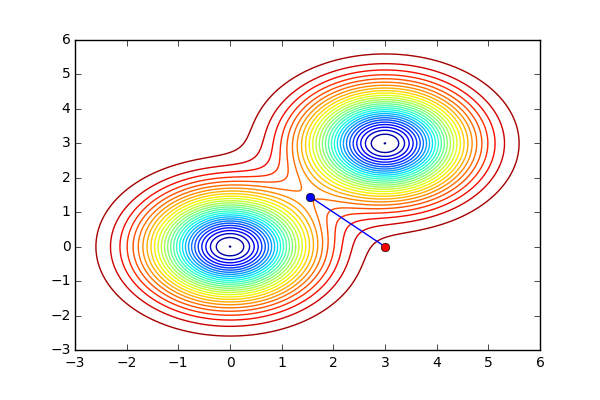
\includegraphics[width=7cm]{../Figures/Q1/normals.png}
  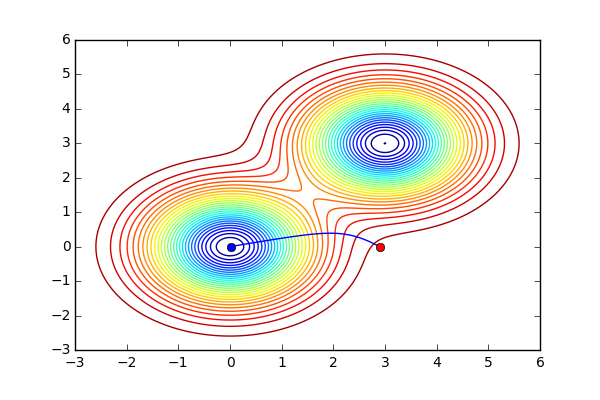
\includegraphics[width=7cm]{../Figures/Q1/normals2.png}
\caption{$f : (x,y) \to -e^{-\frac{x^2 + y^2}{2}} - e^{-\frac{(x-3)^2 + (y-3)^2}{2}}$,$x_0 = (4,3.9)$ (top figure) and $x_0 = (4,4)$(bottom figure), $s = 0.1$ and $\epsilon = 10^{-3}$.}
\label{normals}
\end{figure}



\begin{figure}[h!]
  \centering
 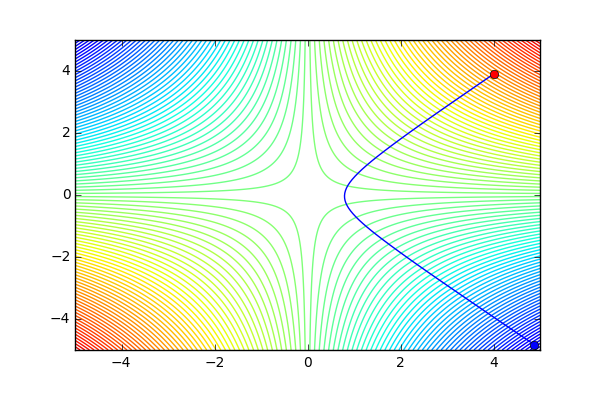
\includegraphics[width=7cm]{../Figures/Q1/nonconv.png}
  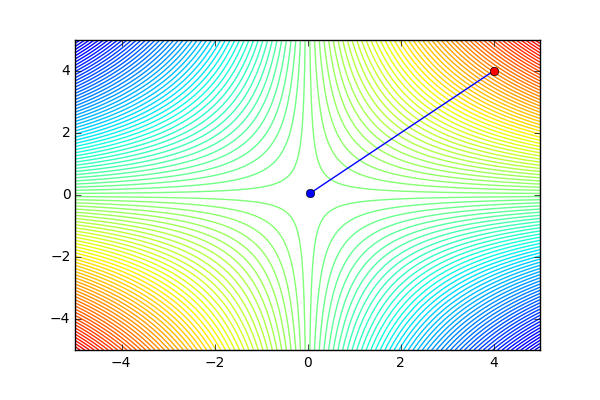
\includegraphics[width=7cm]{../Figures/Q1/nonconv2.png}
\caption{$f : (x,y) \to xy$, $x_0 = (3,0)$ (top figure) and $x_0 = (2.9,0)$(bottom figure), $s = 0.3$ and $\epsilon = 10^{-4}$.}
\label{nonconv}
\end{figure}

\subsubsection{Impact of the step size}

In figure \ref{bowls}, we show the impact of the step size on the convergence of the algorithm, even in the case of a very simple function. For $s$ small enough, the algorithm converges but when we increase $s$, the gradient descent starts cycling, and for even higher values of $s$, it diverges completely.
\begin{figure}[h!]
  \centering
 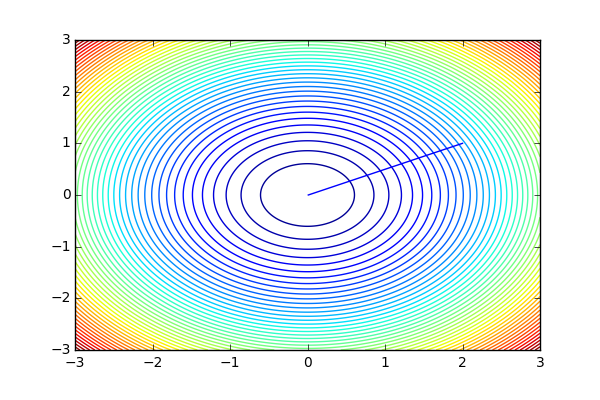
\includegraphics[width=5.5cm,height = 5cm]{../Figures/Q1/bowl.png}
  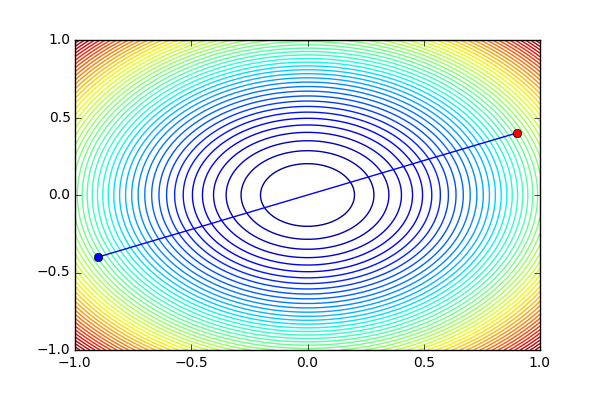
\includegraphics[width=5.5cm,height = 5cm]{../Figures/Q1/bowl2.png}
   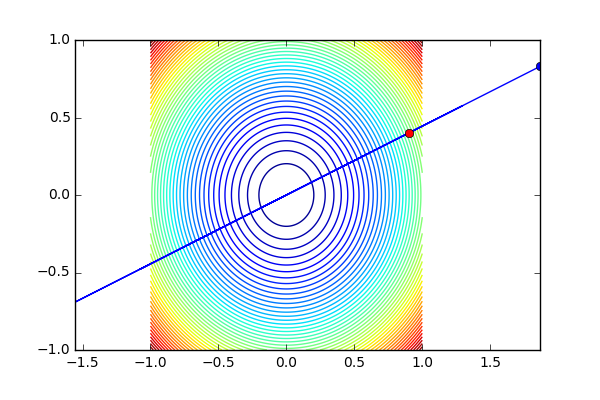
\includegraphics[width=10cm, height = 5cm]{../Figures/Q1/bowl3.png}
\caption{$f : (x,y) \to 10x^2 + 10y^2$, $x_0 = (4,4)$, top to bottom: $s = 0.01, 0.1, 0.11$ and $\epsilon = 0.01$.}
\label{bowls}
\end{figure}

\subsection{Impact of the convergence criterion}
We also noticed that the computational time seems to grow rapidly when $\epsilon \to 0$. However, reasonably small values for $\epsilon$ are needed in order to ensure that the algorithm does not get stuck at a saddle point (in the interest of concision, we did not plot these results, and we refer the reader to our figures \ref{normals} and \ref{nonconv} for examples of saddle points).

\subsection{Numerical Gradient}
\label{numGrad}
We implemented a function {\tt numericalGradient}  that takes the parameters:
\begin{enumerate}[-]
\item A scalar function $f: \mathbb{R}^n \mapsto \mathbb{R}$.
\item An value $x \in \mathbb{R}^n$ at which we wish to compute the gradient
\item Finite difference size $\eta > 0$ (taken as small as possible).
\end{enumerate}
 {\tt gradientDescent} returns an array of $n$ numbers, corresponding to gradient of $f$ at $x$.
 To do that, we use the fact that $(\nabla f (x) )_i = \frac{\partial f}{\partial x_i}|_x = \lim_{\eta \to 0} \frac{f(x + \eta e_i) - f(x)}{\eta} $.
 
 Let us denote $(\widetilde{\nabla_{\eta}}f)(x)$ the numerical gradient given by our algorithms. For $\eta = 0.5$,  and $x = (1,2)$, this gives us the following gradients:

\begin{center}
  \begin{tabular}{| c  | c |r |}
    \hline
 $f$ & $(\nabla f) (x)$ & $(\widetilde{\nabla_\eta}f)(x)$\\ \hline
 $(x,y) \to x^2 + y^2$ & $(2, 4) $  & $(2.5, 4.5)$ \\ \hline
 $ (x,y) \to xy$ &    $ (2,1) $ & $(2.0,1.0)$  \\ \hline
 $(x,y) \to -e^{-\frac{x^2 + y^2}{2}}$& $ \approx (0.082, 0.164)$  & $( 0.076, 0.111)$\\
    \hline
  \end{tabular}
\end{center}

We notice that decreasing $\eta$ to $\eta' = 0.01$ increases the precision of the results. Another way to increase the precision is to take the middle of the finite differences: 
$\frac{\partial f}{\partial x_i}|_x \approx  \frac{f(x + \eta e_i / 2) - f(x -  \eta e_i / 2)}{\eta}$.

\begin{center}
  \begin{tabular}{| c  | c |r |r |}
    \hline
 $f$ & $(\nabla f) (x)$ &  $(\widetilde{\nabla_{\eta'}}f)(x)$ \\ \hline
 $(x,y) \to x^2 + y^2$ & $(2, 4) $  & $(2.01, 4.01)$\\ \hline
 $ (x,y) \to xy$ &    $ (2,1) $ &$(2.0, 1.0)$ \\ \hline
 $(x,y) \to -e^{-\frac{x^2 + y^2}{2}}$& $ \approx (0.082, 0.164)$   &  $(0.082, 0.163)$\\
    \hline
  \end{tabular}
\end{center}

\subsection{Comparison with existing optimization methods}
\label{comparison}
We use the {\tt scipy.optimize.fmin\_bfgs} method to benchmark our algorithm performance. The performance measure is the number of calls to the function. 
We consider three cases corresponding to figure \ref{bowl}, figure \ref{normals} (top case) and figure \ref{nonconv} (bottom case).

\begin{center}
  \begin{tabular}{| c  | r |r |}
    \hline
 Case & {\tt gradientDescent} &  {\tt fmin\_bfgs}  \\ \hline
 $1$ & $57$  & $28$\\ \hline
 $2$ &    $ 21 $ &$3$ \\ \hline
 $3$ & $41$   &  $2$\\
    \hline
  \end{tabular}
\end{center}

We see that in most cases, the scipy algorithm performs better than our {\tt gradientDescent}. This is likely to be due to a better choice of step sizes (compared to our fixed steps, which can be highly inefficient). However, similarly to our solver, it sometimes does not converge to the global minimum.